% This is part of Un soupçon de mathématique sans être agressif pour autant
% Copyright (c) 2015
%   Laurent Claessens
% See the file fdl-1.3.txt for copying conditions.

\begin{exercice}[\ldots\ldots/4]\label{exo2smath-0252}

\begin{wrapfigure}{r}{8.0cm}
    \vspace{-1.5cm}
        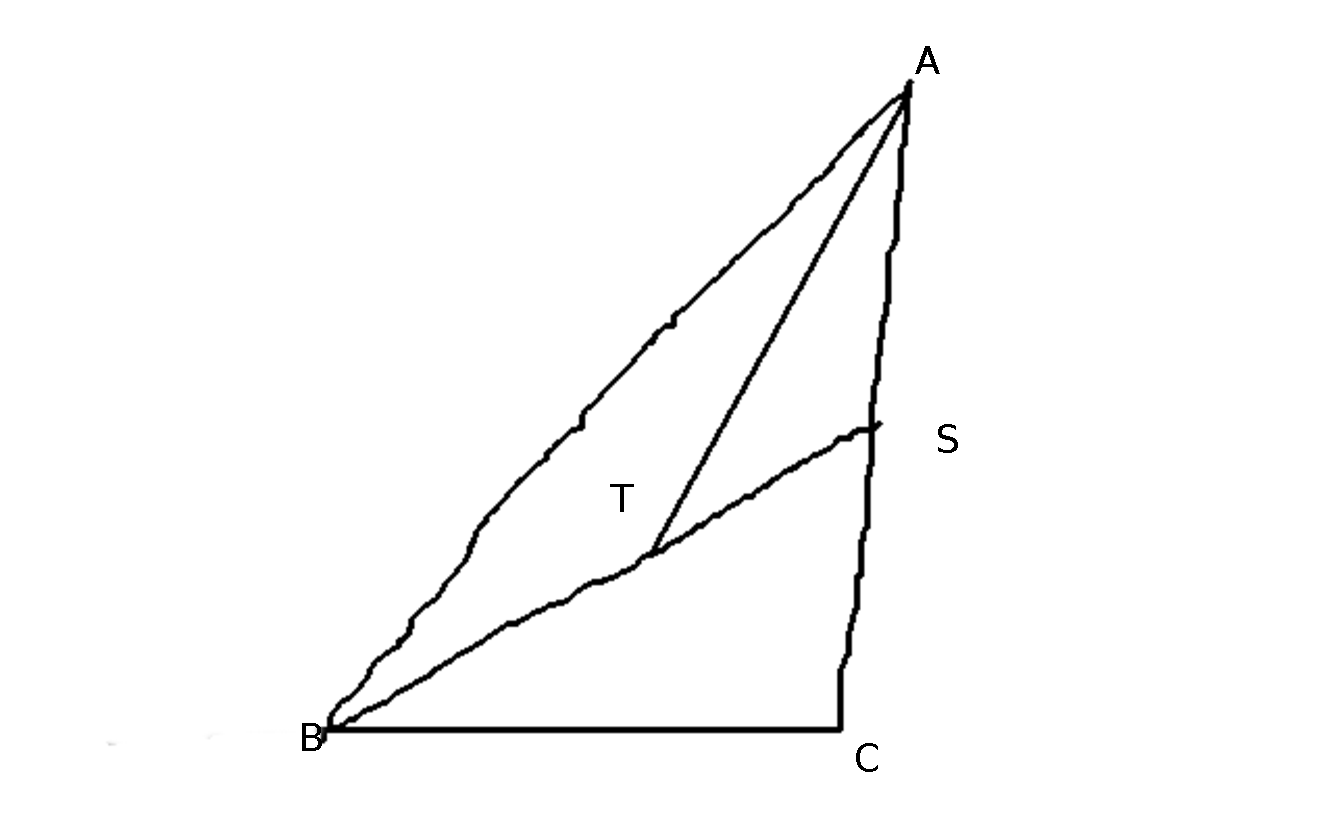
\includegraphics[width=8cm]{LBGPooLcyawW.pdf}
\end{wrapfigure}

    Ajouter des codages de telle sorte que l'aire du triangle \( STA\) représente \( 25\%\) de l'aire du triangle \( ABC\).

    Justifier en citant des propriétés vues au cours.

    \vspace{2cm}

\corrref{2smath-0252}
\end{exercice}
